% 为了增强本研究的鲁棒性,我们在不同的显著性水平下检验了突变点的识别结果,发现在0.0005到0.05的置信度水平下,都只能识别出本研究发现的两个突变点(1978与2001)。
In order to enhance the robustness of this study, we tested the identification results of mutation points at different significance levels.
Our results that only two mutation points (1978 and 2001) could be identified at the confidence level of $0.0005$ to $0.05$ (Figure~\ref{fig:sensitivity}).

% 我们同样使用一些流行的断点识别方法检验了Pettitt的断点识别结果。它们的名称、结果、参考论文可以在表中找到。所有的结果在第二个断点的识别上几乎是一致的(2000年),而第一个断点也仅有3年的差异(1975年与1978年)。
We have also employed a series of popular breakpoint detection methods to validate the results obtained through the Pettitt test. The names of these methods, their respective results, and the references to the pertinent literature can be found in the accompanying table~\ref{table:breakpoint-detection-methods}. A consensus was observed among all methods regarding the identification of the second breakpoint, which consistently emerged around the year 2000. There was a minor variation of three years in the identification of the first breakpoint, pinpointed either in 1975 or 1978.

% 我们综合考虑每个时间段的年份数量后,选择了较为居中的、识别出1977年作为第一个断点的 Pettitt 方法。但可以看得出,本研究所依赖的断点识别结果,对于算法选择的鲁棒性也足够强。
After a thorough evaluation, we opted for the Pettitt method, which identified 1977 as the first breakpoint. This decision was influenced by our intent to ensure a balanced distribution of the number of years across each identified period. The consistency in the identification of breakpoints, especially the second one, across different methods underscores the robustness of our findings, attesting to their insensitivity to the choice of the breakpoint detection algorithm. This robustness reinforces the credibility and reliability of our analyses and conclusions, reflecting the methodological rigor embedded in our study.

\begin{table}[h!]
    \centering
    \begin{tabularx}{\textwidth}{llll}
        \toprule
        \textbf{Method} & \textbf{Breakpoints} & \textbf{Parameters$^*$} & \textbf{Reference} \\
        \midrule
        Generalized ESD Test & 1975, 1978, 2001 & No & \cite{matteson2014} \\
        Pettitt Method & 1978, 2001 & No & \cite{pettitt1979} \\
        Pelt & 1975, 2000 & $pen=0.05$ & \cite{killick2012} \\
        Binary Segmentation & 1975, 2000 & $bkp=2$ & \cite{bai1997} \\
        Bottom-Up Segmentation & 1975, 2000 & $bkp=2$ & \cite{keogh2001} \\
        \bottomrule
    \end{tabularx}
    \footnotesize{$pen$: Penalty coefficient; $bkp$: Number of breakpoints. $No$: Non-parametric test.}
    \caption{Comparison of different breakpoints detection methods}\label{table:breakpoint-detection-methods}
\end{table}


% 此外,我们讨论了在指标中没有体现的水库流量变化,在所有水库(图 x)中,我们分析了10个先后建成的枢纽水库,发现水库在 governance transforming regime 之后开始增强其调度的水平
In addition, we analyzed the changes of reservoir flow that are not reflected in the IWGI.\ Among all the reservoirs (Figure~\ref{fig:reservoirs}), we focused on $9$ major reservoirs built successively and find that the reservoirs began to enhance their variability after the governance transforming regime, suggesting a higher level of regulating (Figure~\ref{fig:conveyance}).

Last, we tried our best to strengthen the period of this study despite the limitations of time span of the multiple-source dataset. We calculated the IWGI from 2003 to 2017 by using data from Yellow River Water Resources Bulletin to extend the study period. Since our results suggest no significant regime change (Figure~\ref{fig:recent}), we think it is robust that the YRB experienced two significant water governance regime changes in 1978 and 2001, without further changing since 21th century.

\begin{figure}[tb]
    \centering
    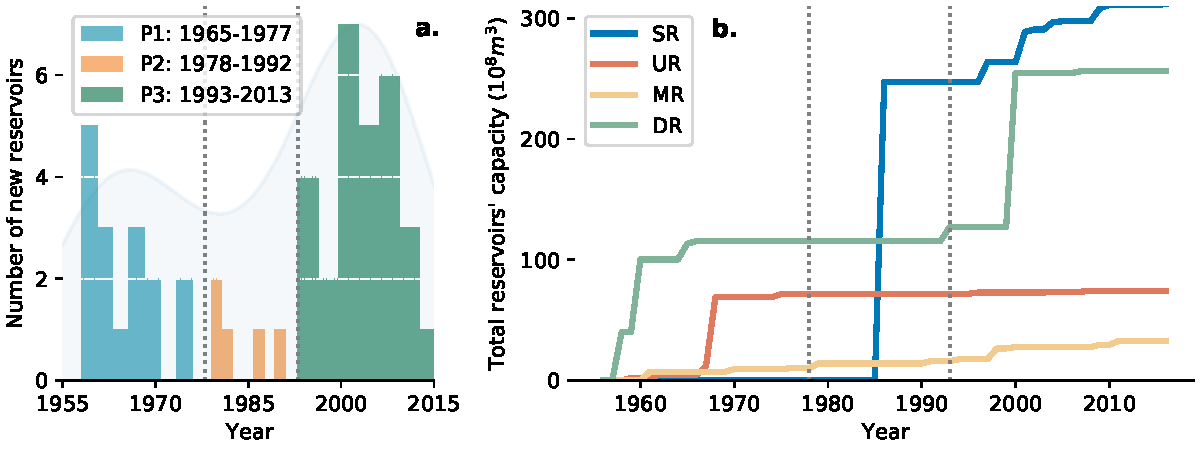
\includegraphics[width=0.6\linewidth]{sup/reservoirs.pdf}
    \caption{
          Numbers of new reservoirs in each year.
    }\label{fig:reservoirs}
\end{figure}

\begin{figure}
    \centering
    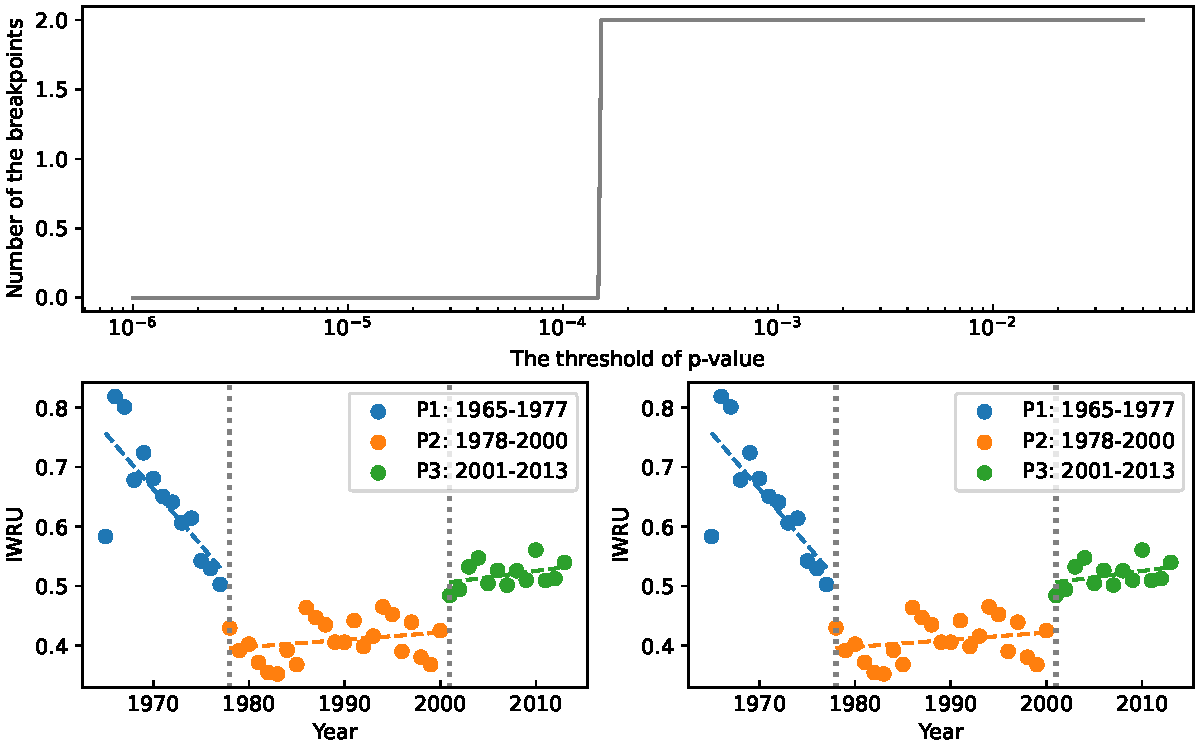
\includegraphics[width=\linewidth]{sup/sensitivity.pdf}
    \caption{
          Sensitivity analysis of the threshold of p-values.
          \textbf{A.} number of breakpoints in different p-values, the scheme with two-breakpoints are the dominant situation.
          \textbf{B.} Threshold of p-values \(\alpha=0.0005\).
          \textbf{C.} Threshold of p-values \(\alpha=0.05\).
    }\label{fig:sensitivity}
\end{figure}


\begin{figure}[htb]
    \centering
    \includegraphics[width=0.8\textwidth]{sup/conveyance.png}
    \caption{Monthly conveyance flow differences of the reservoirs mainly for managing and regulating the whole basin and their variability}\label{fig:conveyance}
\end{figure}


\begin{figure}[!htb]
	\centering
	\includegraphics[width=0.8\textwidth]{sup/robustness.png}
	\caption{Recent years' IWGI changes calculated by data from Yellow River Water Resources Bulletin. No significant changing point exists}\label{fig:recent}
\end{figure}
